\chapter{Aggregate Commit with Verification} % (fold)
\label{cha:A Protocol for Commitment Tree Generation}
	In the previous chapter, we saw that SHIA limits the adversary's ability to manipulate the aggregation result with the tightest bound possible.
	SHIA does not require prior knowledge of network topology and works on hierarchical sensor network which might include multiple malicious sensor nodes, with only suboptimal congestion overhead.
	SHIA helps the sensor node verify, its reported sensor reading was aggregated correctly or not, by an an aggregate node.
	If an an aggregate node has tampered with the reported sensor reading then the relevant sensor node can detect the tampering and raise an alarm.
	But SHIA does not help detecting and revoking the malicious aggregate node from the network.
	We develop the protocol which identifies the malicious aggregate node in the network.
	% which is built on top of commitment tree generation of SHIA mentioned in the previous chapter.
	
	The high level idea of the aggregate commit with verification scheme is, all the leaves in the aggregation tree sends the signature of its data-item signed by itself, in addition to the data-item.
	The aggregate node proceeds to the aggregation only after verifying all the received the data-items.
	The aggregate node signs its payload in addition to its data-item as described in the following sections.

\section{Signing the Data-Item}
	Here, we describe structure of the data-item, how it is different from the label structure of SHIA and rational behind it.

	\begin{definition}
		\label{def:data-item}
		A commitment tree is a binary tree where each vertex has an associated data-item representing the data that is passed on to its parent. The data-items have the following format:

		$\hspace{100pt}$ $<$id, count, value, commitment$>$
	\end{definition}
	Where id is the unique ID of the node; count is the number of leaf vertices in the subtree rooted at this vertex; value is the SUM aggregate computed over all the leaves in the subtree and commitment is a cryptographic commitment.
	We remove the complement field from the label structure Defined \ref{def:label}. 
	We think sending the complement filed is redundant. 
	The complement field is used by the base station (the querier according to SHIA), before the result checking phase, to verify SUM + COMPLEMENT = $n \cdot r$; where $n$ is the number of nodes in the network, $r$ is the upper bound on the allowed sensor readings.
	We can achieve the similar upper bound without sending the complement field.
	As the querier knows $n, r$ and it gets SUM from the root of the aggregation tree.
	If SUM $> n \cdot r$, then the base station knows some node or nodes in the network reported out of range readings. 

	There is one vertex $s_{0}$ for each sensor node $s$, which we call the leaf vertex of $s$.
	The data-item for leaf vertex $s_{0}$ is defined according to Equation \ref{eq:leaf-vertex} and associated signature to it is defined according to Equation \ref{eq:signature-leaf-vertex}.
	\begin{equation}
		\label{eq:leaf-vertex}
		s_{0}\ =\ <s_{id}, 1, s_{value}, H(N||1||s_{value})>
	\end{equation}
	\begin{equation}
		\label{eq:signature-leaf-vertex}
		Sign(s_{0}) = E_{K_{s}}(H(s_{0}))
	\end{equation}
	where $H$ is a collision resistant hash function, $K_{s}$ is the private key of $s$, $N$ is the query nonce.
	In aggregate commit with verification scheme, in addition to sending the data-item, each sensor node sends the signature of the data-item to its parent.
	The parent node verifies all the received signature and then proceeds to the aggregation.
	
	\subsection{Security Analysis}
		\begin{itemize}
			\item A sensor node has the proof for the sent data-item and can not claim sending the different data-item to its parent in the future.
			\item Each data-item has an associated signature to it, which helps an aggregate node verify the authenticity of the data-item.
			\item The parent node has the proof for the received data-item, and can not claim receiving different data-items form its children in the future.
		\end{itemize}

\section{Signing the Commitment Payload}
		We define commitment payload based on the commitment forest Defined in \ref{def:commitment-forest}.
	\begin{definition}
		A \textbf{commitment payload} is a set of data-items of the root vertices of the trees in the outgoing commitment forest.
	\end{definition}
	% We use the term payload for commitment payload and the term forest for the commitment forest.
	For brevity, we use the term forest, payload instead of commitment forest, commitment payload respectively.

	In addition to sending all the data-items with their respective signatures, an aggregate node sends an additional signature to its parent, which is a signature of all the data-items in its payload.
	% Each sensor node signs all the data-items in its commitment payload before sending it to its parent.
	% to prove the fact that it has verified all the data-items in its commitment forests.
	For example, for the aggregation tree shown in Figure \ref{fig:Palm aggregation tree}, the payload of sensor node $C$ is show in Figure \ref{fig:commitment-tree-example-1}.
			\begin{figure}[h!]
				\centering
				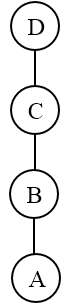
\includegraphics[scale = 0.5]{images/palm-aggregation-tree.png}\\
				\caption{Palm aggregation tree}
				\label{fig:Palm aggregation tree}
			\end{figure}
		% $C$ receives $B_{1}$, $Sign(B_{1})$ from $B$.
		% And $C$'s commitment forest is show in Figure \ref{fig:Commitment forest of C}.
		% $B_{1} = <B_{id}, 2, B_{value}, H(N||2||B_{value}||A_{0}||B_{0})>$; $Sign(B_{1}) = E_{K_{B}}(H(B_{1}))$\\
		% 	\begin{figure}[h!]
		% 		\centering
		% 		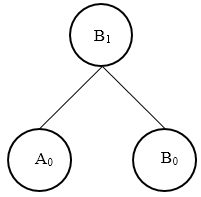
\includegraphics[scale = 0.5]{images/commitment-forest-of-C.png}\\
		% 		\caption{$C$'s commitment forest }
		% 		\label{fig:Commitment forest of C}
		% 	\end{figure}\\
		The sensor node $C$ sends all the data-items in its payload with their signatures to $D$.
		Furthermore, $C$ sends the signature of its payload $Sign(C_{p})$ to $D$.\\
		$B_{1} =\ <B_{id}, 2, B_{value}, H(N||2||B_{value}||A_{0}||B_{0})>$; $Sign(B_{1}) = E_{K_{B}}(H(B_{1}))$\\
		$C_{0} =\ <C_{id}, 1, C_{value}, H(N||1||C_{value})>$; $Sign(C_{0}) = E_{K_{C}}(H(C_{0}))$\\
		\textcolor{red}{$Sign(C_{p}) =\	E_{K_{C}}(H(C_{0} || B_{1}))$}
			\begin{figure}[h!]
				\centering
				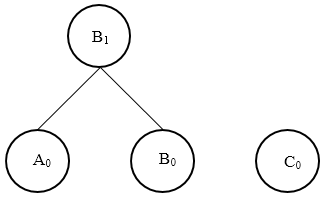
\includegraphics[scale = 0.5]{images/commitment-payload-of-C.png}
				\caption{$C$'s commitment commitment-payload}
				\label{fig:Commitment payload of C}
			\end{figure}
	% Sending an additional signature with all the data-items signifies that a sensor node has verified all the data-items.
	% The basic idea is that the sensor node signs all the data-items it sends to its parent.
	% \textbf{Because of the signature, the sensor node has the proof for the sent data-item.
	% It also prevents the parent or ancestor node from claiming the different received data-item.}
	\subsection{Security Analysis}

	This additional signature signifies the following:
	\begin{itemize}
		\item	An intermediate sensor node has verified all the data-items in its forest before creating its payload.
		\item From the parent node perspective, it has received all the verified data-items from the signer node and not from anywhere else.
		% \item From the parent or ancestor node perspective, it has received all the verified data-items from its children and not from anywhere else.
	\end{itemize}

	\section{Commitment Tree Generation}
	For the given aggregation tree the commitment forest is built as follows.
	Leaf sensor nodes in the aggregation tree create their leaf vertex by creating data-items and their respective signatures according to Equation \ref{eq:leaf-vertex}, \ref{eq:signature-leaf-vertex} which they send it to their parent as a payload in the aggregation tree.
	Each internal sensor node $I$\ in the aggregation tree also creates their leaf vertex and its signature.
	In addition, $I$\ receives the payload from each of its children which creates the forest for $I$.
	Once $I$ verifies all the received signatures, it merges all the data-items in its forest with same count value to create its payload.
	Note that we can determine the height of the commitment tree from the count value.

	Suppose $I$ have to create its payload by merging $i$ data-items $D_{1}$, $D_{2}$, $\dotsc$, $D_{i}$ in its forest.
	First, $I$ verifies the received signatures $Sign(D_{1})$, $Sign(D_{2})$, $\dotsc$, $Sign(D_{i})$.
	Once verified, $I$ starts merging the data-items as follows.
	Let $c$ be the smallest count value in $I$'s forest.
	The sensor node $I$ finds two data-items $D_{1},D_{2}$ in its forest with the same count value $c$ and merges them into a new data-item with the count of $c+1$.
	% \textcolor{red}{add figure}
	It repeats the process until no two data-items in its forest have the same count value.
	An example of generating the payload by merging the data-items in the forest for the sensor node $A$ in Figure \ref{fig:at} is illustrated in the following example.
	% \ref{fig:commitment-tree-example-1}, \ref{fig:commitment-tree-example-2}, \ref{fig:commitment-tree-example-3}, \ref{fig:commitment-tree-example-4}.
			\begin{exmp} The commitment-payload generation process for node $A$ of Figure \ref{fig:at} is shown here.\\
				\begin{figure}[h!]
					\centering
					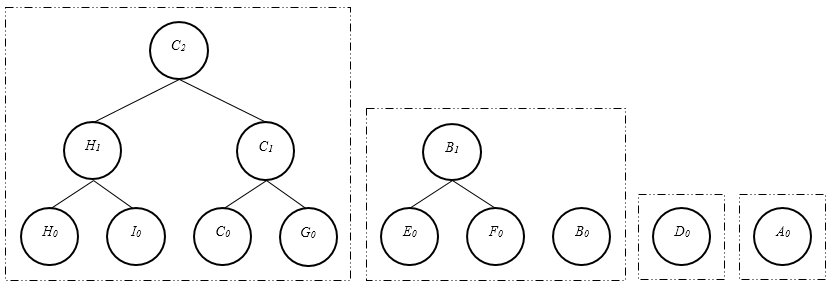
\includegraphics[scale = 1]{images/commitment-tree-example-1.png}\\
					\caption{$A$ receives $C_{2}$ from $C$, $(B_{1},B_{0})$ from $B$, $D_{0}$ from $D$ and generates $A_{0}$. The commitment payload received from a given sensor node is indicated by dashed-line box.}
					\label{fig:commitment-tree-example-1}
				\end{figure}\\
				$A_{0} = <A_{id}, 1, A_{value}, H(N||1||A_{value})>$; $Sign(A_{0}) = E_{K_{A}}(H(A_{0}))$ \\
				$D_{0} = <D_{id}, 1, D_{value}, H(N||1||D_{value})>$; $Sign(D_{0}) = E_{K_{D}}(H(D_{0}))$\\
				$B_{0} = <B_{id}, 1, B_{value}, H(N||1||B_{value})>$; $Sign(B_{0}) = E_{K_{B}}(H(B_{0}))$\\
				$B_{1} = <B_{id}, 2, B_{value}, H(N||2||B_{value}||E_{0}||F_{0})>$; $Sign(B_{1}) = E_{K_{B}}(H(B_{1}))$\\
				\textcolor{red}{$Sign(B_{P}) = E_{K_{B}}(H(B_{0} || B_{1}))$}\\
				$C_{2} = <C_{id}, 4, C_{value}, H(N||4||C_{value})||H_{1}||C_{1})>$; $Sign(C_{2}) = E_{K_{C}}(H(C_{2}))$\\
				\begin{figure}[h!]
					\centering
					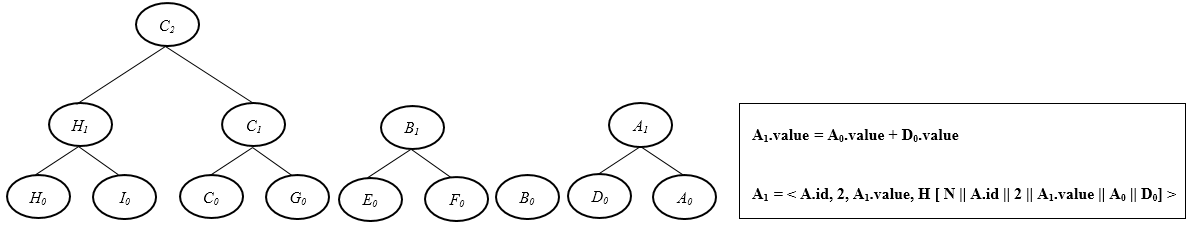
\includegraphics[scale = 1]{images/commitment-tree-example-2.png}\\
					\caption{First Merge: $A_{1}$ vertex created by A.}
					\label{fig:commitment-tree-example-2}
				\end{figure}\\
				$A_{1} = <A_{id}, 2, A_{1value}, H(N||2||A_{1value}||A_{0}||D_{0})>$; $Sign(A_{1}) = E_{K_{A}}(H(A_{1}))$\\
				where $A_{1value} = A_{value} + D_{value} $
				\begin{figure}[h!]
					\centering
					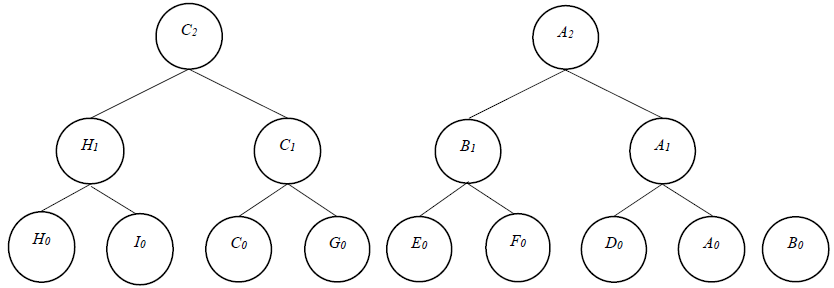
\includegraphics[scale = 1]{images/commitment-tree-example-3.png}\\
					\caption{Second Merge: $A_{2}$ vertex created by A.}
					\label{fig:commitment-tree-example-3}
				\end{figure}\\
				$A_{2} = <A_{id}, 4, A_{2value}, H(N||4||A_{2value}||B_{1}||A_{1}) >$; $Sign(A_{2}) = E_{K_{A}}(H({A_{2}}))$\\
				where $A_{2value} = B_{1value} + A_{1value} $
				\begin{figure}[h!]
					\centering
					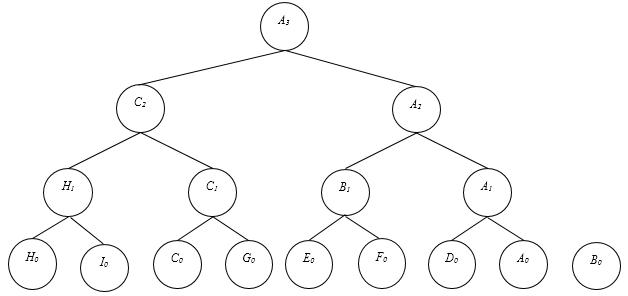
\includegraphics[scale = 1]{images/commitment-tree-example-4.png}\\
					\caption{Third Merge: $A_{3}$ vertex created by A.}
					\label{fig:commitment-tree-example-4}
				\end{figure}\\
				$A_{3} = <A_{id},8, A_{3value},H(N||8||A_{3value}||C_{2}||A_{2})>$; $Sign(A_{3}) = E_{K_{A}}(H(A_{3}))$\\
				$A_{3value} = A_{2value} + C_{2value}$;
			\end{exmp}
% chapter A Protocol for Commitment Tree Generation (end)

% Talk about the certificates:
	
% 	How many certificates does $A$ need to know in this example ?
% 	In the above example, $A$ need to know $D,B,C's$ certificate to verify their signatures.
% 	But if we use SHIA'a approach of creating commitment tree then $A$ need to know $E's$ certificate as well.
% 	Hence, being root in as many tree as possible is the more efficient.
\section{Bandwidth Analysis}
	For a given forest with $n$ leaf vertices, has at most $\log n$ data-items in its payload.
	It has at most $(\log n) +1$ signatures in its payload.
	The highest possible count value is $\log n$, as all the trees are binary. 

	An intermediate sensor node $S$ with $n$ descendants has at most $\log(n+1)$ data-items with their respective $\log(n+1)$ signatures in its payload.
	$S$ might need to send its payload signature $Sign(S_{p})$ to its parent.
	$S$ has to send a payload with $\log(n+1)$ data-items and $\log(n+1) +1$ signatures to its parent in the aggregation tree.
	Hence, sending  signatures of the data-items causes $O(\log n)$ overhead in the network. 

\section{Performance Analysis}
	In addition to calculating the data-items, each sensor node need to do $O(\log n)$ amount of extra work as it needs to calculate and verify $O(\log n)$ signatures. 

	% Computation cost: Needs to calculate that many signatures. Needs to verify that many signatures.
	% Need to know that many certificates.

\section{Applications}
		The signature based aggregation scheme can be applied to do the \textbf{voting} in the network.
		And voting scheme can be used to solve many sensor network problems.
		For example, voting can be used to design the distributed algorithm for selecting a cluster head or node revocation system.
		In the voting scheme, following are the major security concerns: 
		\begin{itemize}
			\item The aggregate node needs to know that the vote is coming from the legit voter, no other voter is impersonating the vote of the legit voter.
			\item Only the intended aggregate node should be able to verify the vote.
			\item The aggregate node should not be able to tamper with the votes. 
			\item The aggregate node needs the proof that it aggregated the verified votes.
			\item The voter need the proof for which vote it sent to its aggregator.
		\end{itemize}
		For example, the base station wants to know the overall vote-count in the network.
		To do so, all the leaf nodes send their votes and the signature of their votes to their respective aggregate nodes in the network.
		The aggregate nodes receive votes with their signatures from all of their children voters.
		The aggregate nodes verify all the votes and count those votes.
		Then they forward the count and the signature of that count signed by the aggregate node to their respective parent in the aggregation tree.
		This process is repeated until the final count and its signature, is sent to the base station by the root of the aggregation tree.
				
	\textbf{Node power level},
	\textbf{Surveillance Application}
